\begin{myConceptSteps}{To find the $x$- and $y$-intercepts of a line from its graph\dots}
    \myStep{plot}{
        Plot the points where the line crosses the $x$- and $y$-axes. 
        There are one or two points.
    }
    \myStep{find}{Find the coordinates of those points.}
    \myStep{$x$-intercept}{
        The point on the $x$-axis has a $y$-coordinate of 0,
        so its coordinates are $(h,0)$, where $h$ is some number. 
        You may write the $x$-intercept either as 
        the point $(h,0)$ or just as the number $h$ (whatever it is).
    }
    \myStep{$y$-intercept}{
        The point on the $y$-axis has an $x$-coordinate of 0,
        so its coordinates are $(0,k)$, where $k$ is some number.
        You may write the $y$-intercept either as 
        the point $(0,k)$ or just as the number $k$ (whatever it is).
    }
\end{myConceptSteps}

\myBlankExample{1.5in}{
    Find $x$- and $y$-intercepts of this line.
    \begin{center}
        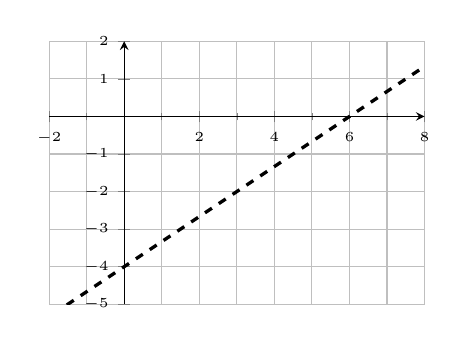
\begin{tikzpicture}
            \begin{axis}[
                width=2.5in,
                grid=both,
                axis x line = middle,axis y line = middle,
                axis equal image,
                xtick distance = 2, ytick distance = 1, 
                minor x tick num = 1,
                xmin = -2, xmax=8,
                ymin = -5, ymax=2,
                tick label style = {font=\tiny},
                ]
                \addplot[dashed,style={line width=1.2pt},no marks, samples=3, domain=-3:10 ] expression { (2/3)*x -4 };
            \end{axis}
        \end{tikzpicture}
    \end{center}
}

\myBlankExample{1.5in}{
    Find $x$- and $y$-intercepts of this line.
    \begin{center}
        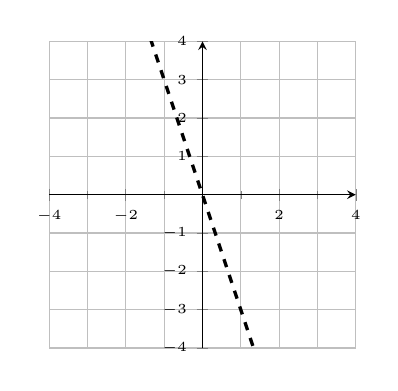
\begin{tikzpicture}
            \begin{axis}[
                width=2.5in,
                grid=both,
                axis x line = middle,axis y line = middle,
                axis equal image,
                xtick distance = 2, ytick distance = 1, 
                minor x tick num = 1,
                xmin = -4, xmax=4,
                ymin = -4, ymax=4,
                tick label style = {font=\tiny},
                ]
                \addplot[dashed,style={line width=1.2pt},no marks, samples=3, domain=-3:10 ] expression { -3*x };
            \end{axis}
        \end{tikzpicture}
    \end{center}
}

\myBlankExample{1.2in}{
    Find $x$- and $y$-intercepts of this line.
    \begin{center}
        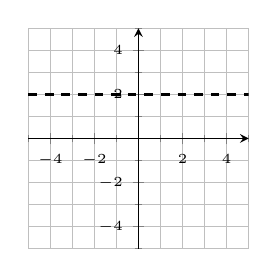
\begin{tikzpicture}
            \begin{axis}[
                width=2.in,
                grid=both,
                axis x line = middle,axis y line = middle,
                axis equal image,
                xtick distance = 2, ytick distance = 2, 
                minor tick num = 1,
                xmin = -5, xmax=5,
                ymin = -5, ymax=5,
                tick label style = {font=\tiny},
                ]
                \addplot[dashed,style={line width=1.2pt}, no marks, samples=100, domain=-5:5, ] expression { 2 };
            \end{axis}
        \end{tikzpicture}
    \end{center}
}

\myBlankExample{1.25in}{
    Find $x$- and $y$-intercepts of this line.
    \begin{center}
        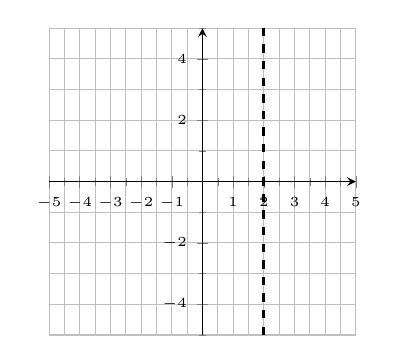
\begin{tikzpicture}
            \begin{axis}[
                width=2.5in,
                grid=both,
                axis x line = middle,axis y line = middle,
                axis equal image,
                xtick distance = 1, ytick distance = 2, 
                minor tick num = 1,
                xmin = -5, xmax=5,
                ymin = -5, ymax=5,
                tick label style = {font=\tiny},
                ]
                \addplot +[mark=none,dashed,style={line width=1.2pt}, black] coordinates {(2, -5) (2, 5)};
            \end{axis}
        \end{tikzpicture}
    \end{center}
}
